\documentclass[cjk,dvipdfmx,10pt,compress,%
hyperref={bookmarks=true,bookmarksnumbered=true,bookmarksopen=false,%
colorlinks=false,%
pdftitle={第 121 回 関西 Debian 勉強会},%
pdfauthor={倉敷・のがた・佐々木・かわだ},%
%pdfinstitute={関西 Debian 勉強会},%
pdfsubject={資料},%
}]{beamer}

\title{第 121 回 関西 Debian 勉強会\\(10 周年記念会)}
\subtitle{$\sim$発表資料$\sim$}
\author[かわだ てつたろう]{{\large\bf 倉敷・のがた・佐々木・かわだ・おおつき}}
\institute[Debian JP]{{\normalsize\tt 関西 Debian 勉強会}}
\date{{\small 2017 年 3 月 19 日}}

%\usepackage{amsmath}
%\usepackage{amssymb}
\usepackage{graphicx}
\usepackage{moreverb}
\usepackage[varg]{txfonts}
\AtBeginDvi{\special{pdf:tounicode EUC-UCS2}}
\usetheme{Kyoto}
\def\museincludegraphics{%
  \begingroup
  \catcode`\|=0
  \catcode`\\=12
  \catcode`\#=12
  \includegraphics[width=0.9\textwidth]}
%\renewcommand{\familydefault}{\sfdefault}
%\renewcommand{\kanjifamilydefault}{\sfdefault}
\begin{document}
\settitleslide
\begin{frame}
\titlepage
\end{frame}
\setdefaultslide

\begin{frame}[fragile]
  \frametitle{Disclaimer}
  \begin{itemize}
  \item 疑問、質問、ツッコミ、茶々、\alert{大歓迎}
  \item その場でインタラクティブにどうぞ
  \item ハッシュタグ \#kansaidebian
  \end{itemize}
\end{frame}

\takahashi[100]{祝 10 周年}

%\begin{frame}[fragile]
%\frametitle{Agenda}
%\tableofcontents
%\end{frame}

\section{事前課題}
\takahashi[50]{事前課題}

\begin{frame}[fragile]
  \frametitle{事前課題}
  \begin{block}{今回の事前課題}
    \begin{description}
    \item 関西 debian 勉強会にいつから参加されましたか?
    \end{description}
  \end{block}
\end{frame}

\begin{frame}[fragile]
  \frametitle{nogajun}
    \begin{block}{関西 debian 勉強会にいつから参加されましたか?}
        \begin{description}
            \item 第0回は出られなかったので第1回からのはず
            \url{http://www.nofuture.tv/diary/20070331.html#p01}
        \end{description}
    \end{block}
\end{frame}

\begin{frame}[fragile]
  \frametitle{ipv6waterstar}
    \begin{block}{関西 debian 勉強会にいつから参加されましたか?}
        \begin{description}
            \item
        \end{description}
    \end{block}
\end{frame}

\begin{frame}[fragile]
  \frametitle{znz}
    \begin{block}{関西 debian 勉強会にいつから参加されましたか?}
        \begin{description}
            \item 調べて見たら第2回が初参加のようでした。
        \end{description}
    \end{block}
\end{frame}

\begin{frame}[fragile]
  \frametitle{YukiharuYABUKI}
    \begin{block}{関西 debian 勉強会にいつから参加されましたか?}
        \begin{description}
            \item 最初から
        \end{description}
    \end{block}
\end{frame}

\begin{frame}[fragile]
  \frametitle{yosuke\_san}
    \begin{block}{関西 debian 勉強会にいつから参加されましたか?}
        \begin{description}
            \item 2015 年 6 月 だったかな?
        \end{description}
    \end{block}
\end{frame}

\begin{frame}[fragile]
  \frametitle{Katsuki Kobayashi}
    \begin{block}{関西 debian 勉強会にいつから参加されましたか?}
        \begin{description}
            \item それ以前にも一度参加した事がありましたが、
              第106回(2016-01-24)あたりからはわりと継続して参加してるようです。
        \end{description}
    \end{block}
\end{frame}

\begin{frame}[fragile]
  \frametitle{murase\_syuka }
    \begin{block}{関西 debian 勉強会にいつから参加されましたか?}
        \begin{description}
            \item 初参加は2008年ごろ?年に1回くるか来ないかペースですけど:−)
        \end{description}
    \end{block}
\end{frame}

\begin{frame}[fragile]
  \frametitle{uwabami}
    \begin{block}{関西 debian 勉強会にいつから参加されましたか?}
        \begin{description}
            \item 日記をさかのぼってみたら、初参加が2008年5月でした.
              どこでこの勉強会を知ったのかイマイチ思い出せないのですが、
              2007年に神戸に移動してから、人と話す機会が少なくて寂しかっ
              たんだと思います(笑)
        \end{description}
    \end{block}
\end{frame}

\begin{frame}[fragile]
  \frametitle{gdevmjc}
    \begin{block}{関西 debian 勉強会にいつから参加されましたか?}
        \begin{description}
            \item 第1回
        \end{description}
    \end{block}
\end{frame}

\begin{frame}[fragile]
  \frametitle{Say\_no}
    \begin{block}{関西 debian 勉強会にいつから参加されましたか?}
        \begin{description}
            \item 第3回から
        \end{description}
    \end{block}
\end{frame}

\begin{frame}[fragile]
  \frametitle{t3rkwd}
    \begin{block}{関西 debian 勉強会にいつから参加されましたか?}
        \begin{description}
            \item 2009年9月の第27回から。
        \end{description}
    \end{block}
\end{frame}

\begin{frame}[fragile]
  \frametitle{Takaya Yamashita}
    \begin{block}{関西 debian 勉強会にいつから参加されましたか?}
        \begin{description}
            \item 第1回からです。途中参加できていません。
        \end{description}
    \end{block}
\end{frame}

\begin{frame}[fragile]
  \frametitle{lurdan}
    \begin{block}{関西 debian 勉強会にいつから参加されましたか?}
        \begin{description}
            \item わりと最初の頃のはず
        \end{description}
    \end{block}
\end{frame}


\takahashi[120]{次}

\takahashi[50]{矢吹さん} % 仮の題目

\takahashi[120]{次}

\takahashi[50]{山下さん} % 仮の題目

\takahashi[50]{そんな\\こんなで}
\takahashi[120]{次}

\takahashi[50]{10 年間の参加人数を振り返る}

\begin{frame}[fragile]
  \frametitle{10 年間の参加人数を振り返る}
  \begin{figure}
    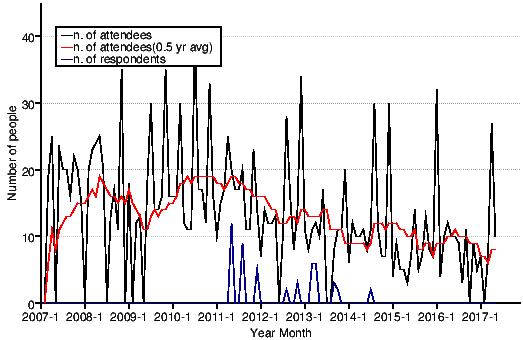
\includegraphics[scale=0.5]{image201703-kansai/memberanalysis/kansai.png}
  \end{figure}
\end{frame}

\begin{frame}[fragile]
  \frametitle{過去の話題を振り返る}
   \begin{itemize} 
    \item 第 1 回開催から第 121 回まで
    \item 2014 年に何があった?
   \end{itemize} 
\end{frame}

\begin{frame}[fragile]
  \frametitle{2007 年の話題}

    \begin{table}
        \begin{center}
          \begin{tabular}{|l|c|p{16em}|}
            \hline
            開催年月   & 参加人数 & 内容 \\
            \hline
            2007年3月  & 19       & 開催にあたり \\
            2007年4月  & 25       & goodbye、youtube、プロジェクトトラッカー\\
            2007年6月  & 23       & 社会契約、テーマ、debian/rules、bugreport\\
            2007年7月  & 20前後   & OSC-Kansai \\
            2007年8月  & 20       & Inkscape、patch、dpatch\\
            2007年9月  & 16       & ライブラリ、翻訳、debtorrent\\
            2007年10月 & 22       & 日本語入力、SPAMフィルタ\\
            2007年11月 & 20前後   & KOF \\
            2007年12月 & 15       & 忘年会、iPod touch\\
            \hline
          \end{tabular}
        \end{center}
    \end{table}
\end{frame}

\begin{frame}[fragile]
  \frametitle{2008 年の話題}
    \begin{table}
        \begin{center}
          \begin{tabular}{|l|c|p{16em}|}
            \hline
            開催年月   & 参加人数 & 内容 \\
            \hline
            2008年2月  & 20       & PC Cluster, GIS, \TeX \\
            2008年3月  & 23       & bug report, developer corner, GPG \\
            2008年4月  & 24       & coLinux, Debian GNU/kFreeBSD, sid \\
            2008年5月  & 25       & ipv6, emacs, ustream.tv\\
            2008年6月  & 20       & pbuilder, hotplug, ssl\\
            2008年8月  & 13       & coLinux \\
            2008年9月  & 17       & debian mentors, ubiquity, DFSG\\
            2008年10月 & 11       & cdbs,cdn.debian.or.jp \\
            2008年11月 & 35       & KOF \\
            2008年12月 & ?        & TeX資料作成ハンズオン\\
            \hline
          \end{tabular}
        \end{center}
    \end{table}
\end{frame}

\begin{frame}[fragile]
  \frametitle{2009 年の話題}
    \begin{table}
        \begin{center}
          \begin{tabular}{|l|c|p{16em}|}
            \hline
            開催年月   & 参加人数 & 内容 \\
            \hline
            2009年1月  & 18       & DMCK, LT \\
            2009年3月  & 12       & Git \\
            2009年4月  & 13       & Installing sid, Mancoosi, keysign \\
            2009年6月  & 18       & Debian Live, bash\\
            2009年7月  & 30?      & OSC2009Kansai \\
            2009年8月  & 14       & DDTSS, lintian \\
            2009年9月  & 14       & reportbug, debian mentors\\
            2009年10月 & 16       & gdb, packaging \\
            2009年11月 & 35       & KOF2009 \\
            2009年12月 & 16       & GPS program, OpenStreetMap \\
            \hline
          \end{tabular}
        \end{center}
    \end{table}
\end{frame}

\begin{frame}[fragile]
  \frametitle{2010 年の話題}
    \begin{table}
        \begin{center}
          \begin{tabular}{|l|c|p{16em}|}
            開催年月   & 参加人数 & 内容 \\
            \hline
            2010年1月  & 16       & Xen, 2010年企画 \\
            2010年2月  & 16       & レンタルサーバでの利用, GAE \\
            2010年3月  & 30?      & OSC2010Kobe \\
            2010年4月  & 12       & デスクトップ環境, 正規表現 \\
            2010年5月  & 11       & ubuntu, squeeze \\
            2010年6月  & 11       & debhelper7, cdbs, puppet \\
            2010年7月  & 40?      & OSC2010Kyoto \\
            2010年8月  & 17       & emdebian, kFreeBSD \\
            2010年9月  & 17       & タイルWM \\
            2010年10月 & 12       & initramfs, debian live \\
            2010年11月 & 33       & KOF2010 \\
            2010年12月 & 14       & Proxmox, annual review \\
            \hline
          \end{tabular}
        \end{center}
    \end{table}
\end{frame}

\begin{frame}[fragile]
  \frametitle{2011 年の話題}
    \begin{table}
        \begin{center}
          \begin{tabular}{|l|c|c|p{16em}|}
            \hline
            開催年月  & 参加 & 回答 & 内容 \\
            \hline
            2011年1月 &10    & 0    & BTS, kFreeBSD\\
            2011年2月 &15    & 0    & pbuilder, Squeezeリリースパーティ\\
            2011年3月 &17    & 0    & ライセンス, ドキュメント\\
            2011年4月 &25    & 0    & OSC Kansai@Kobe \\
            2011年5月 &20    &12    & vi, dpkg \\
            2011年6月 &17    & 0    & vcs-buildpackage\{svn, git\}, IPv6\\
            2011年7月 &17    & 0    & OSC Kansai@Kyoto \\
            2011年8月 &20    & 9    & パッケージ作成ハンズオン\\
            2011年9月 &11    & 0    & vcs-buildpackage\{bzr, git\}\\
            2011年10月&11    & 0    & Emacs, vim 拡張のDebianパッケージ, 翻訳\\
            2011年11月&23    & 0    & KOF 2011\\
            2011年12月&13    & 5    & NMプロセス, BTS\\
            \hline
          \end{tabular}
        \end{center}
    \end{table}
\end{frame}

\begin{frame}[fragile]
  \frametitle{2012 年の話題}
    \begin{table}
        \begin{center}
          \begin{tabular}{|l|c|c|p{20em}|}
            \hline
            開催年月  & 参加 & 回答 & 内容 \\
            \hline
            2012年1月 & 7    &0     & Debian温泉合宿 \\
            2012年2月 &14    &0     & autofs+pam\_chroot, t-code, Debian Policy \\
            2012年3月 &12    &0     & Konoha, t-code, Debian Policy \\
            2012年4月 &12    &0     & フリーソフトウェアと著作権, Konoha, Debian Policy \\
            2012年5月 &13    &0     & DebianとLDAP(頓挫), ITP入門, Debian Policy \\
            2012年6月 & -    &0     & 大統一Debian勉強会 \\
            2012年7月 &10    &0     & DebianとLDAP, Debian Policy \\
            2012年8月 &28    &2     & OSC Kansai@Kyoto \\
            2012年8月 &16    &0     & DebianとKerberos, News from EDOS \\
            2012年9月 & 8    &0     & clang, Debian Policy \\
            2012年10月&14    &3     & 翻訳環境構築, DSAの舞台裏\\
            2012年11月&34    &0     & KOF 2012\\
            2012年12月&12    &0     & Debian on Android, Debian Policy \\
            \hline
          \end{tabular}
        \end{center}
    \end{table}
\end{frame}

\begin{frame}[fragile]
  \frametitle{2013 年の話題}
    \begin{table}
        \begin{center}
          \begin{tabular}{|l|c|c|p{20em}|}
            \hline
            開催年月  & 参加 & 回答 & 内容 \\
            \hline
            2013年1月 & 8    &0     & Drupal, Debian Policy \\
            2013年2月 &11    &6     & Debian Installer, Ruby \\
            2013年3月 &12    &6     & GNOME Shell, GNOME \\
            2013年4月 &10    &0     & リリースノート, AWS \\
            2013年5月 &17    &0     & DebianとUbuntu, Debianの歩き方 \\
            2013年6月 & -    &0     & 大統一Debian勉強会 \\
            2013年7月 &      &0     & OSC 2013 Kansai @ Kyoto\\
            2013年8月 & 8    &3     & puppet \\
            2013年9月 &11    &2     & サウンドシステム, dgit \\
            2013年10月&11    &0     & ALSA, git-buildpackage \\
            2013年11月&20    &0     & KOF 2013 \\
            2013年12月& 6    &0     & 2013年の振り返りと2014年の企画, 忘年会 \\
            \hline
          \end{tabular}
        \end{center}
    \end{table}
\end{frame}

\begin{frame}[fragile]
  \frametitle{2014 年の話題 (もくもくしすぎ) }
    \begin{table}
        \begin{center}
          \begin{tabular}{|l|c|c|p{20em}|}
            \hline
            開催年月  & 参加 & 回答 & 内容 \\
            \hline
            2014年1月 &12    &0     & LT, もくもくの会 \\
            2014年2月 &10    &0     & もくもくの会 \\
            2014年3月 &10    &0     & 3D プリンティング, もくもくの会 \\
            2014年4月 &11    &0     & kvm, Notmuch Mail \\
            2014年5月 & 8    &0     & もくもくの会 \\
            2014年6月 &11    &2     & systemd, Linuxのドライバメンテナ, \\
                      &      &      & キーサイン \\
            2014年8月 &30    &0     & OSC 2014 Kansai @ Kyoto \\
                      &11    &0     & もくもくの会 \\
            2014年9月 & 7    &0     & もくもくの会 \\
            2014年10月& 7    &0     & もくもくの会 \\
            2014年11月&30    &0     & KOF 2014 \\
                      & 4    &0     & インストーラテスト, もくもくの会 \\
            2014年12月& 9    &0     & 2014年の振り返りと2015年の企画, 忘年会 \\
            \hline
          \end{tabular}
        \end{center}
    \end{table}
\end{frame}

\begin{frame}[fragile]
  \frametitle{2015 年の話題}
    \begin{table}
        \begin{center}
          \begin{tabular}{|l|c|p{20em}|}
            \hline
            開催年月  & 参加人数 & 内容 \\
            \hline
            2015年1月 &5      & Debian Bug Squashing Party \\
                      &5      & Debian の Bug の眺め方, Bug Squash Party \\
            2015年2月 &3      & もくもくの会 \\
            2015年3月 &7      & 某所 VPS を先走って Jessie に上げてみた \\
            2015年4月 &14     & Debian 8 "Jessie" Release Party \\
            2015年5月 &5      & Jessie落穂拾い \\
            2015年6月 &7      & Wheezy→Jessieで踏み抜いた地雷のご紹介 \\
            2015年7月 &13     & OSC 2015 Kansai @ Kyoto \\
            2015年8月 &8      & wiki:Subkeys \\
            2015年9月 &7      & ドイツ、ハイデルベルクで開催されたDebconf15へいってきました \\
            2015年11月&32     & KOF 2015 \\
                      &4      & ライトニングトーク, もくもくの会 \\
            2015年12月&9      & 2015年の振り返りと2016年の企画, 忘年会 \\
            \hline
          \end{tabular}
        \end{center}
    \end{table}
\end{frame}

\begin{frame}[fragile]
  \frametitle{2016 年の話題}
    \begin{table}
        \begin{center}
          {\small
          \begin{tabular}{|l|c|p{20em}|}
            \hline
            開催年月  & 参加人数 & 内容 \\
            \hline
            2016年1月 & 12    & GNUHurdのインストールしてみた。と、Xサーバの立ち上げに挑戦 \\
                      &       & VyOSを入れてAPを構築してみた。\\
            2016年2月 & 10    & 勉強会資料の歩き方 \\
                      &       & 周回遅れでDocker触ってみた \\
            2016年3月 & 10    & systemd に浸かってみる \\
            2016年4月 & 9     & OpenFOAM による数値流体解析 \\
            2016年5月 & 3     & ライトニングトーク \& もくもくの会  \\
            2016年6月 & 11    & Debian パッケージング道場\\
            2016年7月 &       & OSC 2016 @ Kyoto \\
            2016年8月 & 9     & ライトニングトーク \& もくもくの会 \\
            2016年9月 & 5     & 初心者が初めてパッケージをつくってみた \\
                      &       & Let's Encryptのススメ \\
            2016年10月& 7     & sbuild と debci を触ってみた \\
            2016年11月&       & KOF 2016 \\
            2016年12月& 7      & 2016年の振り返りと2017年の企画, 忘年会 \\
            \hline
          \end{tabular}
          }
        \end{center}
    \end{table}
\end{frame}

\begin{frame}[fragile]
  \frametitle{2017 年の話題}
    \begin{table}
        \begin{center}
          \begin{tabular}{|l|c|p{20em}|}
            \hline
            開催年月  & 参加人数 & 内容 \\
            \hline
            2017年1月 & 27    & 関西 Debian 勉強会 + openSUSE Meetup + LILO \& 東海道らぐLT大会 \\
            2017年2月 & 10    & qmakeなQtアプリのdebを作ろうとして試行錯誤した話 \\
            2017年3月 &     & 10 周年記念会 \\
            \hline
          \end{tabular}
        \end{center}
    \end{table}
\end{frame}

\begin{frame}[fragile]
  \frametitle{今後の予定}
  \begin{block}{第122回関西Debian勉強会}
    \begin{itemize}
    \item 日時: 4月30日(日)
    \item 場所: 福島区民センター
    \item 内容: Debian 9 Strech Release Party もしくは CMake
    \end{itemize}
  \end{block}

\end{frame}

\takahashi[30]{ これからもよろしくお願いいたします。 }

\end{document}
%%% Local Variables:
%%% mode: japanese-latex
%%% TeX-master: t
%%% End:
